%% The first command in your LaTeX source must be the \documentclass command.
\documentclass[acmtog]{acmart}
\usepackage[english,ngerman]{babel}
\usepackage[utf8]{inputenc} 

%% \BibTeX command to typeset BibTeX logo in the docs
\AtBeginDocument{%
  \providecommand\BibTeX{{%
    \normalfont B\kern-0.5em{\scshape i\kern-0.25em b}\kern-0.8em\TeX}}}
    
\copyrightyear{2024}
\acmYear{2024}
\citestyle{acmauthoryear}

\usepackage[figurename=Fig.]{caption}
\usepackage{csquotes}
\setcopyright{none}
\makeatletter
\renewcommand{\fnum@figure}{Abb. \thefigure}
\makeatother
\addto\captionsngerman{\renewcommand{\figurename}{Abb.}}
\settopmatter{printacmref=false} % Removes citation information below abstract
\renewcommand\footnotetextcopyrightpermission[1]{} % removes footnote with conference information in first column

\usepackage{minted}

%%
%% end of the preamble, start of the body of the document source.
\begin{document}

%%
%% The "title" command has an optional parameter,
%% allowing the author to define a "short title" to be used in page headers.
\title{Enterprise Architektur-Muster}

%%
%% The "author" command and its associated commands are used to define
%% the authors and their affiliations.
%% Of note is the shared affiliation of the first two authors, and the
%% "authornote" and "authornotemark" commands
%% used to denote shared contribution to the research.
\author{Julian Bruder}
\authornote{Alle Studierenden trugen zu gleichen Teilen zu dieser Arbeit bei.}
\author{Abdellah Filali}
\authornotemark[1]
\author{Luca Franke}
\authornotemark[1]
\affiliation{%
  \institution{Hochschule für Technik, Wirtschaft und Kultur Leipzig (HTWK Leipzig)}
  \streetaddress{Karl-Liebknecht-Str. 132}
  \city{Leipzig}
  \country{Deutschland}
  \postcode{04277}
}
%%
%% By default, the full list of authors will be used in the page
%% headers. Often, this list is too long, and will overlap
%% other information printed in the page headers. This command allows
%% the author to define a more concise list
%% of authors' names for this purpose.
\renewcommand{\shortauthors}{Bruder, Filali, Franke}

%%
%% The abstract is a short summary of the work to be presented in the
%% article.
\begin{abstract}
Blah abstrakt\ldots
\end{abstract}

\maketitle

\section{Einleitung}
% (Beschreibung von Kontext, Problemen, Anforderungen und Zielen)
Mit E-Commerce-Beispiel motivieren

\section{Grundlagen von Enterprise-Architekturen}
Verteilte Systeme \ldots

Architekturen \ldots

Komponenten \ldots

\ldots


\section{Klassische Enterprise-Architekturen}

\subsection{Service-oriented}
Die bisherigen Architekturmuster, wie die Monolithic Architecture waren
durch ihren engen gekoppelten Funktionalitäten charakterisiert.
Jetzt betrachten wir die Service-oriented Architecture (SOA), die als zentrales
Konzept von Dienste (englisch \textit{Services}) betont.

Der Begriff Service-oriented Architecture wurde am 1996 von Roy Schulte und Yefim Natis geprägt, um
 eine Architektur zu beschreiben, die die Logik und Daten in mehrere Anwendungen wiederverwendet.\cite[104]{soa3}

Eine universelle Definition von SOA ist nicht vorhanden, jedoch ist das Konzept
von Dienst ein zentrales Element der Architektur.
Ein Dienst in SOA ist oft grob granuliert und besitzt folgenden Eigenschaften \cite[16]{soa2}\cite[19]{soa4}:
\begin{itemize}
  \item Der Dienst ist eine unabhängige Einheit
  \item Der Dienst ist über einen Namen oder eine Adresse Webbasierte-Technologien erreichbar
  \item Der Dienst verfügt über eine publizierte Schnittstelle
  \item Der Dienst ist durch eine Registry auffindbar
  \item Der Dienst kann zur Laufzeit dynamisch lokalisiert und genutzt werden
\end{itemize}

 Betrachten wir im Folgenden die Hauptbestandteile der SOA, wie die Abb. ~\ref{fig:soa} \cite{soa4} darstellt:
\begin{itemize}
  \item Service Provider: Bietet einen spezifischen Dienst an
  \item Service Bus: Dienst, das die Orchestrierung der Kommunikation zwischen Consumer und Provider gewährleistet
  \item Service Consumer: Nutzt einen bereitgestellten Dienst, dieses kann einen End-User oder ein anderer Dienst sein
  \item Service Registry: Dient als zentrale Sammlung von Meta-Daten über die verfügbare Dienste
\end{itemize}

\begin{figure}[!h]
  \centering
  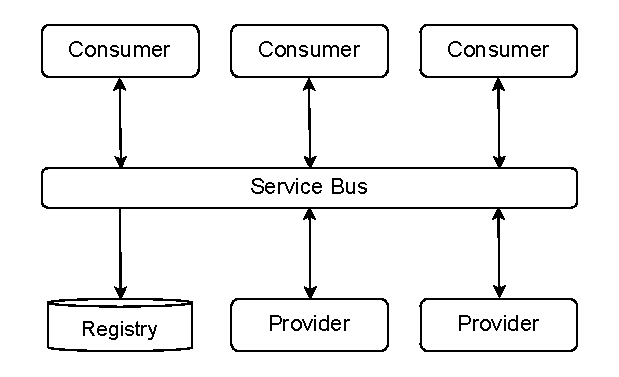
\includegraphics[width=0.8\linewidth]{images/soa/soa.pdf}
  \caption{Aufbau der Service-oriented Architecture}
  \label{fig:soa}
\end{figure}

Die Registry ist eine Sammlung von verfügbaren Diensten und deren Spezifikationen, wo
Provider ihre Dienste registrieren und Consumer Dienste dynamisch zu Laufzeit entdecken können.
Die Provider legen klare, definierte Endpoints und Verträge fest, an denen sich die Consumer
halten müssen, um die Dienste nutzen zu können \cite[23 - 24]{soa4}.

Ein Service Bus, insbesondere ein Enterprise Service Bus (ESB), übernimmt die zentrale
Aufgabe der Orchestrierung der Kommunikation zwischen Provider und Consumer.
Zu den typischen Funktionen eines ESB gehören u.a. das Routing, sowie die
Konvertierung der Nachrichten, falls Dienste unterschiedliche Protokolle für die Kommunikation verwenden \cite[37]{soa4}.

In SOA ist es zusätzlich möglich, ein Broker zu nutzen, um die Kommunikation zwischen
Consumer und Provider zu ermöglichen.\cite[2]{soa5}

Betrachten wir im Folgenden eine mögliche Implementierung der SOA mit einem Broker anhand des E-Commerce-Beispiels.
Dafür definieren wir drei Arten von Services:
\begin{itemize}
  \item \texttt{OrderService}: Ein Dienst, das den gesamtenten Bestellvorgang initiiert
  \item \texttt{PaymentService}: Ein Dienst, das der Bezahlvorgang darstellt
  \item \texttt{ShipmentService}: Ein Dienst, das der Versandvorgang darstellt
\end{itemize}

\begin{figure}[!h]
  \centering
  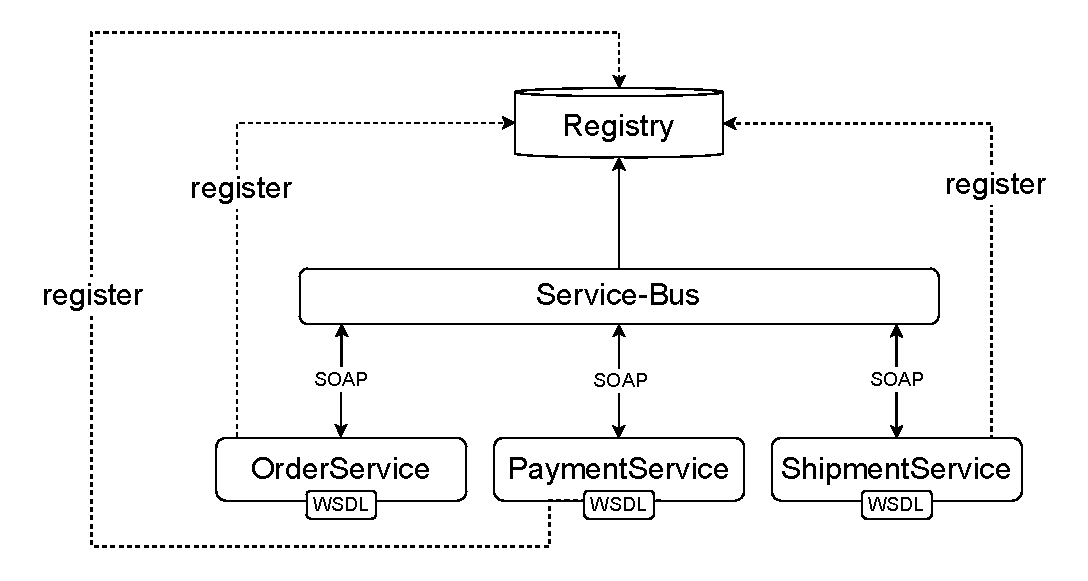
\includegraphics[width=0.8\linewidth]{images/soa/soa-example.pdf}
  \caption{E-Commerce-Beispiel mit Service-oriented Architecture}
  \label{fig:soaecommerce}
\end{figure}

Wie Abbildung \ref{fig:soaecommerce} zeigt, die Dienste\texttt{ShipmentService},
\texttt{PaymentService} und \texttt{OrderService} registrieren ihre Dienste
bei dem \texttt{Registry}.

In diesem Beispiel \texttt{OrderService} konsumiert die beiden anderen Dienste.
 Dieses erfolgt durch Anfragen über den Broker, der die \texttt{Registry} anspricht.
Nach Erhalt der Meta-Daten, der \texttt{OrderService} kann die benötigten Dienste
 gemäß den Interface-Verträge nutzen.

Die vollständige Implementierung des E-Commerce-Beispiels ist bei GitHub \footnote{https://github.com/Beleg-6-EAP/demo-soa-ecommerce} zu finden.

Sollte sich die Implementierung oder die Schnittstellen der Provider ändern, ist
der Consumer nicht davon betroffen, da die Dienste in der \texttt{Registry}
 dynamisch zu Laufzeit lokalisiert und genutzt werden.

Da jeder Service einen spezifischen Dienst anbieten und diese durch eine
 klar definite Schnittstellen, können Dienste unabhängig voneinander
 weiterentwickelt werden, was die kleine autonome Teams ermöglicht.

Außerdem Dienste sind einständig und können getrennt deployt werden,
 was die häufige Auslieferung von Software in kürzere Iterationen ermöglicht.

Skalierung ist hie bei auch möglich, da die Dienste unabhängig voneinander sind.

Ein Nachteil der SOA ist jedoch, dass langfristig Abhängigkeit zwischen den Diensten
entstehen können, besonders wenn die Dienste grob granuliert sind.
\section{Moderne Enterprise-Architekturen}

\subsection{Event-Driven Architecture}
Die Event-Driven Architecture wählt als Basis einen anderen Ausgangspunkt als die bisherigen Architekturmuster.
Während bei letzteren Komponenten Dienste bereitstellen, welche von anderen Komponenten explizit genutzt werden,
verhalten sich Dienst-bereitstellende Komponenten in der Event-Driven Architecture reaktiv,
werden also implizit von Dienst-konsumierenden Komponenten genutzt \cite{garlanShawImplizit}.
Ein System reagiert somit asynchron auf Zustandsänderungen, also Ereignisse in diesem System \cite{eda}.
Die in dieser Architektur minimalen Einheiten, welche Informationen einer Zustandsänderung kapseln, werden \textit{Events} genannt.
Die Idee der impliziten Behandlung von Ereignissen ist nicht neu und taucht erstmals 1994 im von Garlan und Shaw publizierten Papier
\textit{\enquote{An introduction to Software Architecture}} auf.

Betrachten wir im Folgenden die Basis-Bestandteile der Event-Driven Architecture:
\begin{itemize}
  \item Ereignis (englisch \textit{Event}): Kapselt Information einer Zustandsänderung eines Systems
  \item Produzent (englisch \textit{Producer}): Komponente, die Event erzeugt
  \item Herausgeber (englisch \textit{Publisher}): Komponente, die, von Produzenten erzeugte, Events publiziert
  \item Konsument (englisch \textit{Consumer}): Komponente, die auf publizierte Events reagiert
  \item Vermittler (englisch \textit{Mediator}): Komponente zwischen Produzenten und Konsumenten - filtert Events und verteilt diese auf Konsumenten
  \item Event-Bus: Oft auch \textit{Event-Broker} genannt - bietet die Infrastruktur für die Gesamtheit der Vermittler
\end{itemize}
Abstrakt kann ein Event als Vertrag zwischen Produzenten und Konsumenten am Event-Bus betrachtet werden.
Der Konsument nutzt die Spezifikation des Events am Bus, der Produzent implementiert jene Spezifikation.
Abbildung \ref{fig:eda} stellt diesen Vertrag dar.

\begin{figure}[!h]
  \centering
  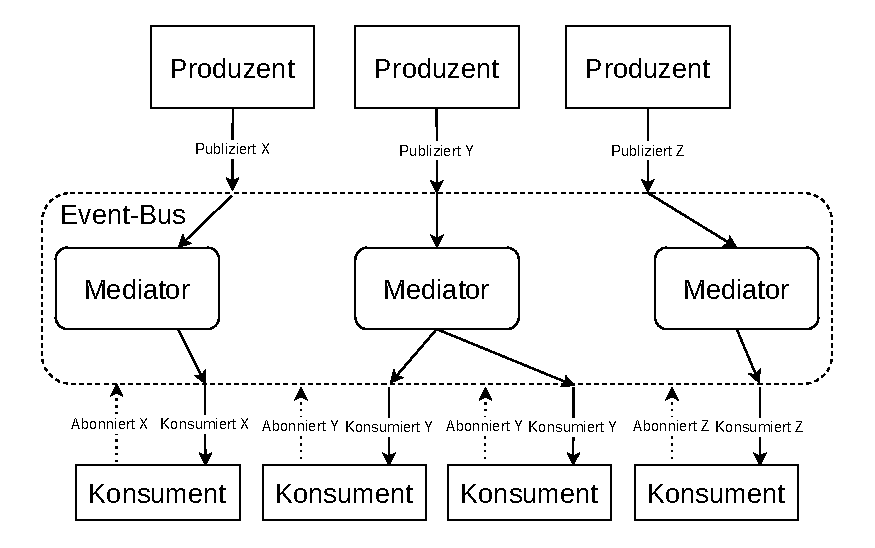
\includegraphics[width=\linewidth]{images/eda/eda.drawio}
  \caption{Vertrag zwischen Produzenten und Konsumenten am Event-Bus}
  \label{fig:eda}
\end{figure}

Durch den Vertrag weisen die Events am Event-Bus starke Kohäsion und somit lose Kopplung auf.
Diese lose Kopplung minimiert nicht nur kaskadierende Fehler, sondern ermöglicht agilen Entwickler-Teams durch klar abgegrenzte Features einfach definierbare Iterationen
- eine Menge von Events, deren Erzeugung und Konsumierung.

Weiter sind Events oft nah an dem, was Ereignisse in realen Prozessen sind, also domain-driven.
Gebündelt ermöglichen obige Punkte die kontinuierliche Auslieferung von Software in kurzen Intervallen.

Außerdem garantiert die asynchrone Behandlung von Ereignissen zusammen mit der loosen Kopplung maximale Skalierung.
Daher sind Event-Driven Architekturen besonders für datenintensive Echtzeit-Anwendungen wie IoT (Internet of Things) und Analytics geeignet \cite{iotEda}.

Betrachten wir erneut das E-Commerce-Beispiel aus der Einleitung.
Dafür definieren wir drei Arten von Events:
\begin{itemize}
  \item \texttt{OrderCreated}: Ein Event, das genau dann erzeugt wird, wenn eine neue Bestellung aufgegeben wird
  \item \texttt{PaymentProcessed}: Ein Event, das genau dann erzeugt wird, wenn der Bezahlvorgang abgeschlossen wird
  \item \texttt{ShipmentInitiated}: Ein Event, das genau dann erzeugt wird, wenn die Bestellung versandt wird
\end{itemize}

Weiter teilen wir die Funktionalität ähnlich wie bei der Microservice-Architektur in die drei verschiedenen Dienste \texttt{OrderService}, \texttt{PaymentService} und \texttt{ShipmentService} auf.

\begin{figure}[!h]
  \centering
  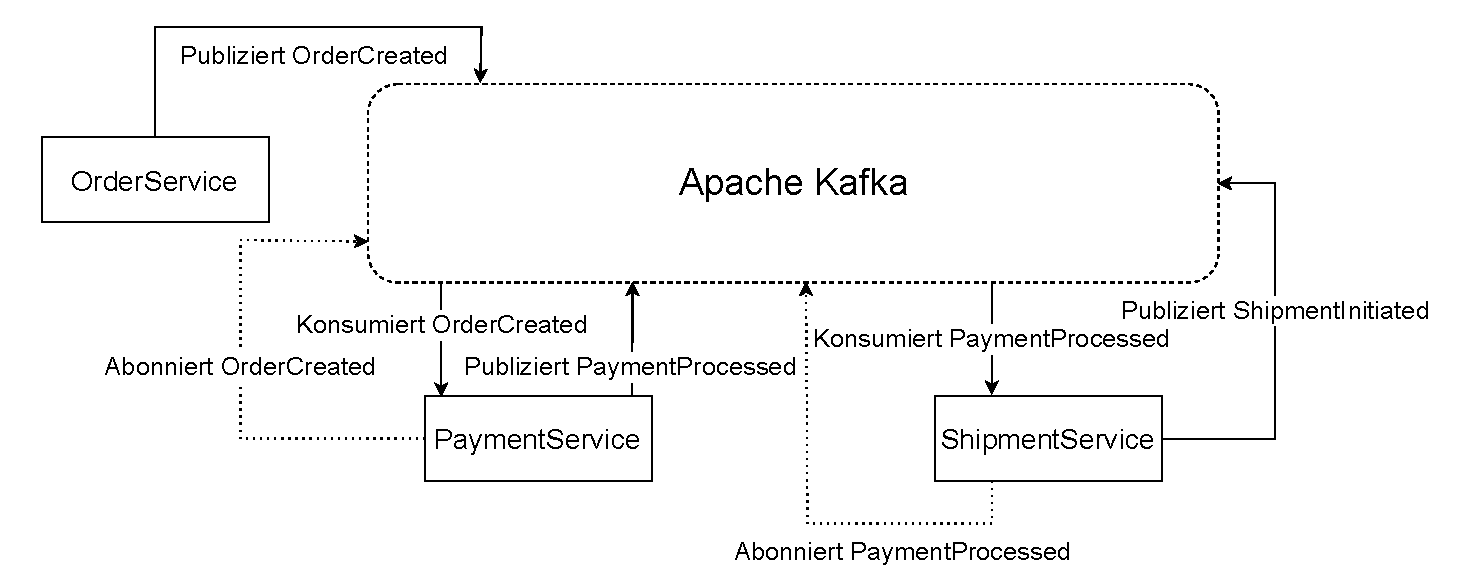
\includegraphics[width=\linewidth]{images/eda/eda-ecommerce.drawio}
  \caption{E-Commerce-Beispiel mit Event-Driven Architecture}
  \label{fig:edaecommerce}
\end{figure}
Wie Abbildung \ref{fig:edaecommerce} zeigt, sind alle drei Dienste Produzenten und Publisher, erzeugen also Events und veröffentlichen diese.
Die Dienste \texttt{PaymentService} und \texttt{ShipmentService} sind zudem Konsumenten,
sodass ersterer auf Events des Typs \texttt{OrderCreated} und zweiterer auf Events des Typs \texttt{ShipmentInitiated} reagiert.
Eine beispielhafte Implementierung des \texttt{PaymentService} mit Apache Kafka als Event-Broker ist im Anhang \ref{app:code:eda:paymentservice} zu finden.
Die vollständige Implementierung des E-Commerce-Beispiels ist bei GitHub \footnote{https://github.com/Beleg-6-EAP/demo-eda-ecommerce} zu finden.

Das Beispiel zeigt, dass die Event-Driven Architektur mit weiteren agilen Strukturen wie Microservices kombiniert werden kann, was die Agilität der Architektur weiter erhöht.
Die damit einhergehende Komplexität stellt teilweise hohe Anforderungen an die Entwickler.
Aufgrund der Asynchronität der Behandlung von Ereignissen ist die Testung des Systems meist schwer und die Fehlerbehandlung essentiell.
Mögliche Problemquellen schließen dabei unter anderem Event-Verlust, erhöhte Latenz und Inkonsistenz ein.
Die hohen Anforderungen an die Entwickler verlangen viel Vertrauen in jene, einer der zentralen Punkte des agilen Manifests \cite{agileManifesto}.
Insgesamt weist die Event-Driven Architecture also eine sehr hohe Agilität auf und ist damit besonders für moderne Software und ihre stetig wechselnden Anforderungen geeignet.

\section{Fallstudien und Praxisbeispiele}
Blah \ldots

\section{Diskussion}

\section{Zusammenfassung und Ausblick}
%(Überblick über die gesamte Arbeit, Rückführung auf Aussagen aus Kapitel 1 durchführen, offene Punkte als neue Forschungsfragen definieren)






\bibliographystyle{ACM-Reference-Format}
\bibliography{main}

\appendix

\section{Code-Beispiele}

\subsection{Event-Driven-Architecture}
\label{app:code:eda:paymentservice}
\begin{listing}[H]
  \tiny
  \inputminted[linenos=true]{java}{code/eda/PaymentService.java}
  \caption{Service-Implementierung des \texttt{PaymentService} in Java Spring Boot 3.4.1 mit Apache Kafka als Event-Broker}
  \label{listing:semigroup}
\end{listing}

\section{Übungsaufgaben}
\subsection{Übungsaufgabe 1 }
Blah \ldots

\end{document}
\endinput
